\documentclass[12pt]{article}

\usepackage[margin=0.8in]{geometry}
\usepackage{graphicx}
\usepackage{float}
\usepackage{amsmath}
\usepackage[nottoc]{tocbibind}
\usepackage{listings}
\usepackage{indentfirst}
\usepackage[hidelinks]{hyperref}
\usepackage{wrapfig}
\usepackage{pdflscape}
\usepackage{xcolor}

%%\setcounter{tocdepth}{3}
%%\setcounter{secnumdepth}{3}


\begin{document}
\begin{titlepage}
\begin{center}


\vspace*{3cm}
\begin{LARGE}
\textbf{EE 413}\\
\vspace{1cm}
\textsc{Term Project}\\
\vspace{1cm}

\begin{Large}
\textsc{Basic Microcontroller \\ \vspace{0.4cm}
Architecture Proposal Report}
\end{Large}
\end{LARGE}
       
\vspace{3cm}

\begin{large}
{\bf Berk Aslan}  \\
2231272 \\
\vspace{1cm}
Submission Date: 23.01.2022 
\end{large}

\vspace{2cm}



\includegraphics[width=0.5\textwidth]{odtumetu}
            
\href{https://eee.metu.edu.tr/}{Electrical - Electronics Engineering}\\
\href{https://metu.edu.tr/}{Middle East Technical University}\\
{Ankara \& Turkey}\\

       
\pagestyle{empty}  
\end{center}
\end{titlepage}


\subsection*{Introduction}

This document is the first report of the EE413 term project, in which we have been assigned to design and implement a basic microcontroller. Microcontroller structure in the project includes an arithmetic logic unit(ALU), logic controller, instruction memory, data memory and output RAM. Throughout the report, proposed architectures for all of this systems will be explained. Prior to them, some overall decisions and timing is explained below.

\subsection*{Overall Decisions and Timing}

The most important aspect of a digital design process is timing. Therefore, before any other thing, we should start with timing.\\

Every modern digital system have some form of the timing counter. In this project, I will use a sequence counter approach. Figure \ref{seq} shows the sequence counter implementation. Figure \ref{timing} in the next page includes a timing example interval. Explanations follow:

\begin{figure}[H]
\centering
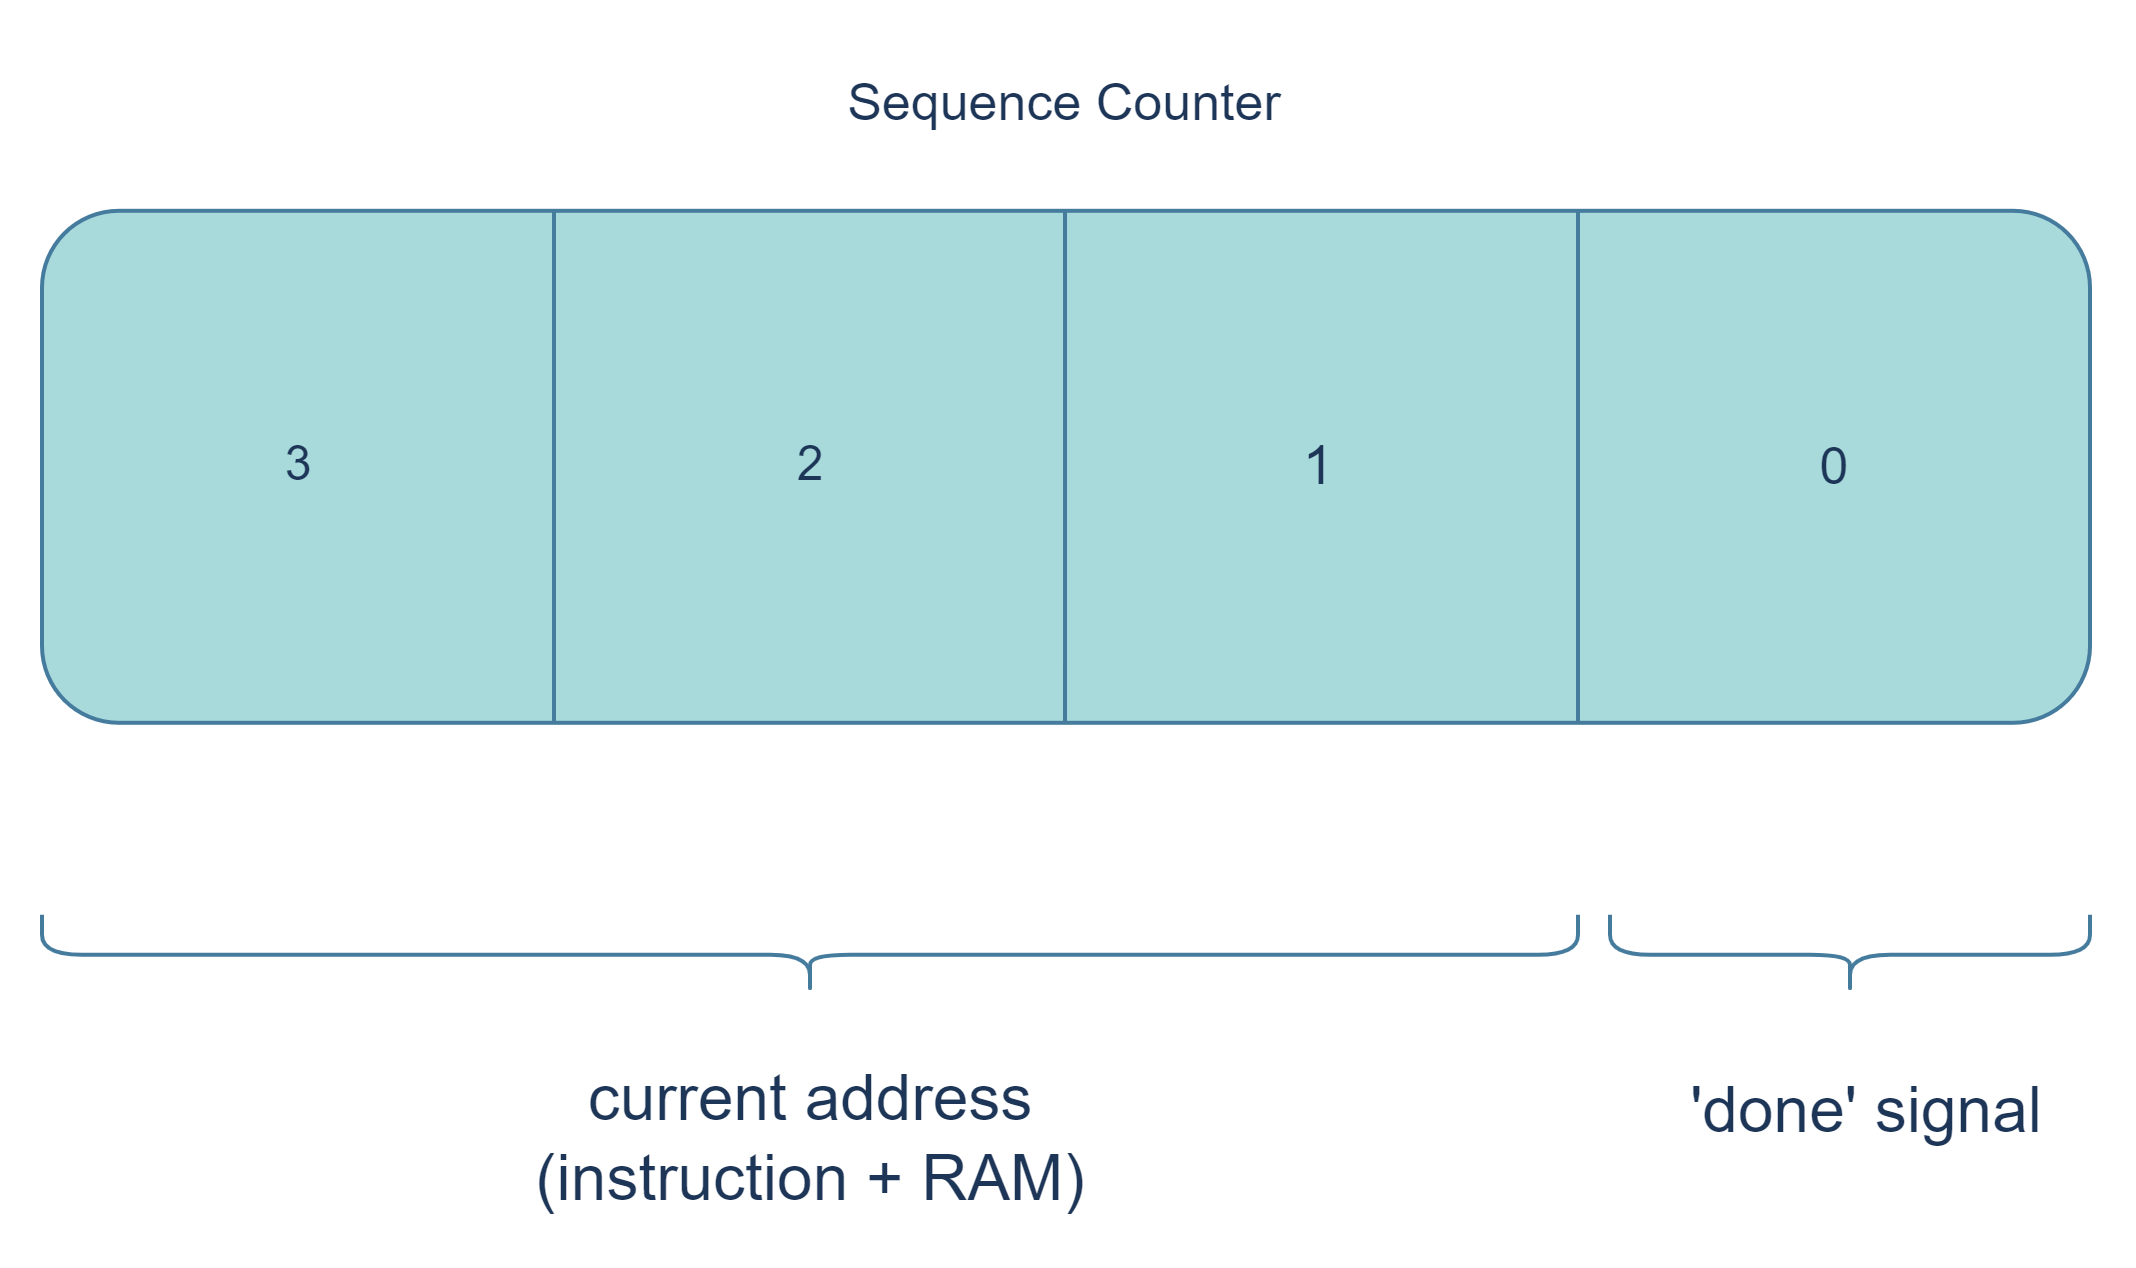
\includegraphics[scale=0.2]{seq.png}
\caption{Sequence Counter}
\label{seq}
\end{figure}

\begin{itemize}
\item Sequence counter starts to count with the \textsl{Start} signal. It is a 4-bit synchronous counter. It counts from 0 to 15. Hence, 8 instructions will be completed in 16 cycles.

\item The MSB 3 bit of the SC holds the current address of the instruction. This address also stands for the RAM address to be written. This part increases with every 2 CLK cycles.

\item  The LSB bit holds for the \textsl{Done} signal. This signal indicates that the operation is done at the ALU part. Instructions can be shifted for the next operation. This signal triggers loading of the instruction memory as will be explained later.

\item In fact, every instruction could be completed in 1 CLK cycle. However, I wanted to stay on the safe side and allocate 2 CLK cycles for every instruction. In case of an improper operation due to the delays, it is also possible to use the second CLK cycle. At this point, it behaves like a safety interval between the instructions.
\end{itemize}

\begin{landscape}
\pagestyle{empty}
\begin{figure}[H]
\centering
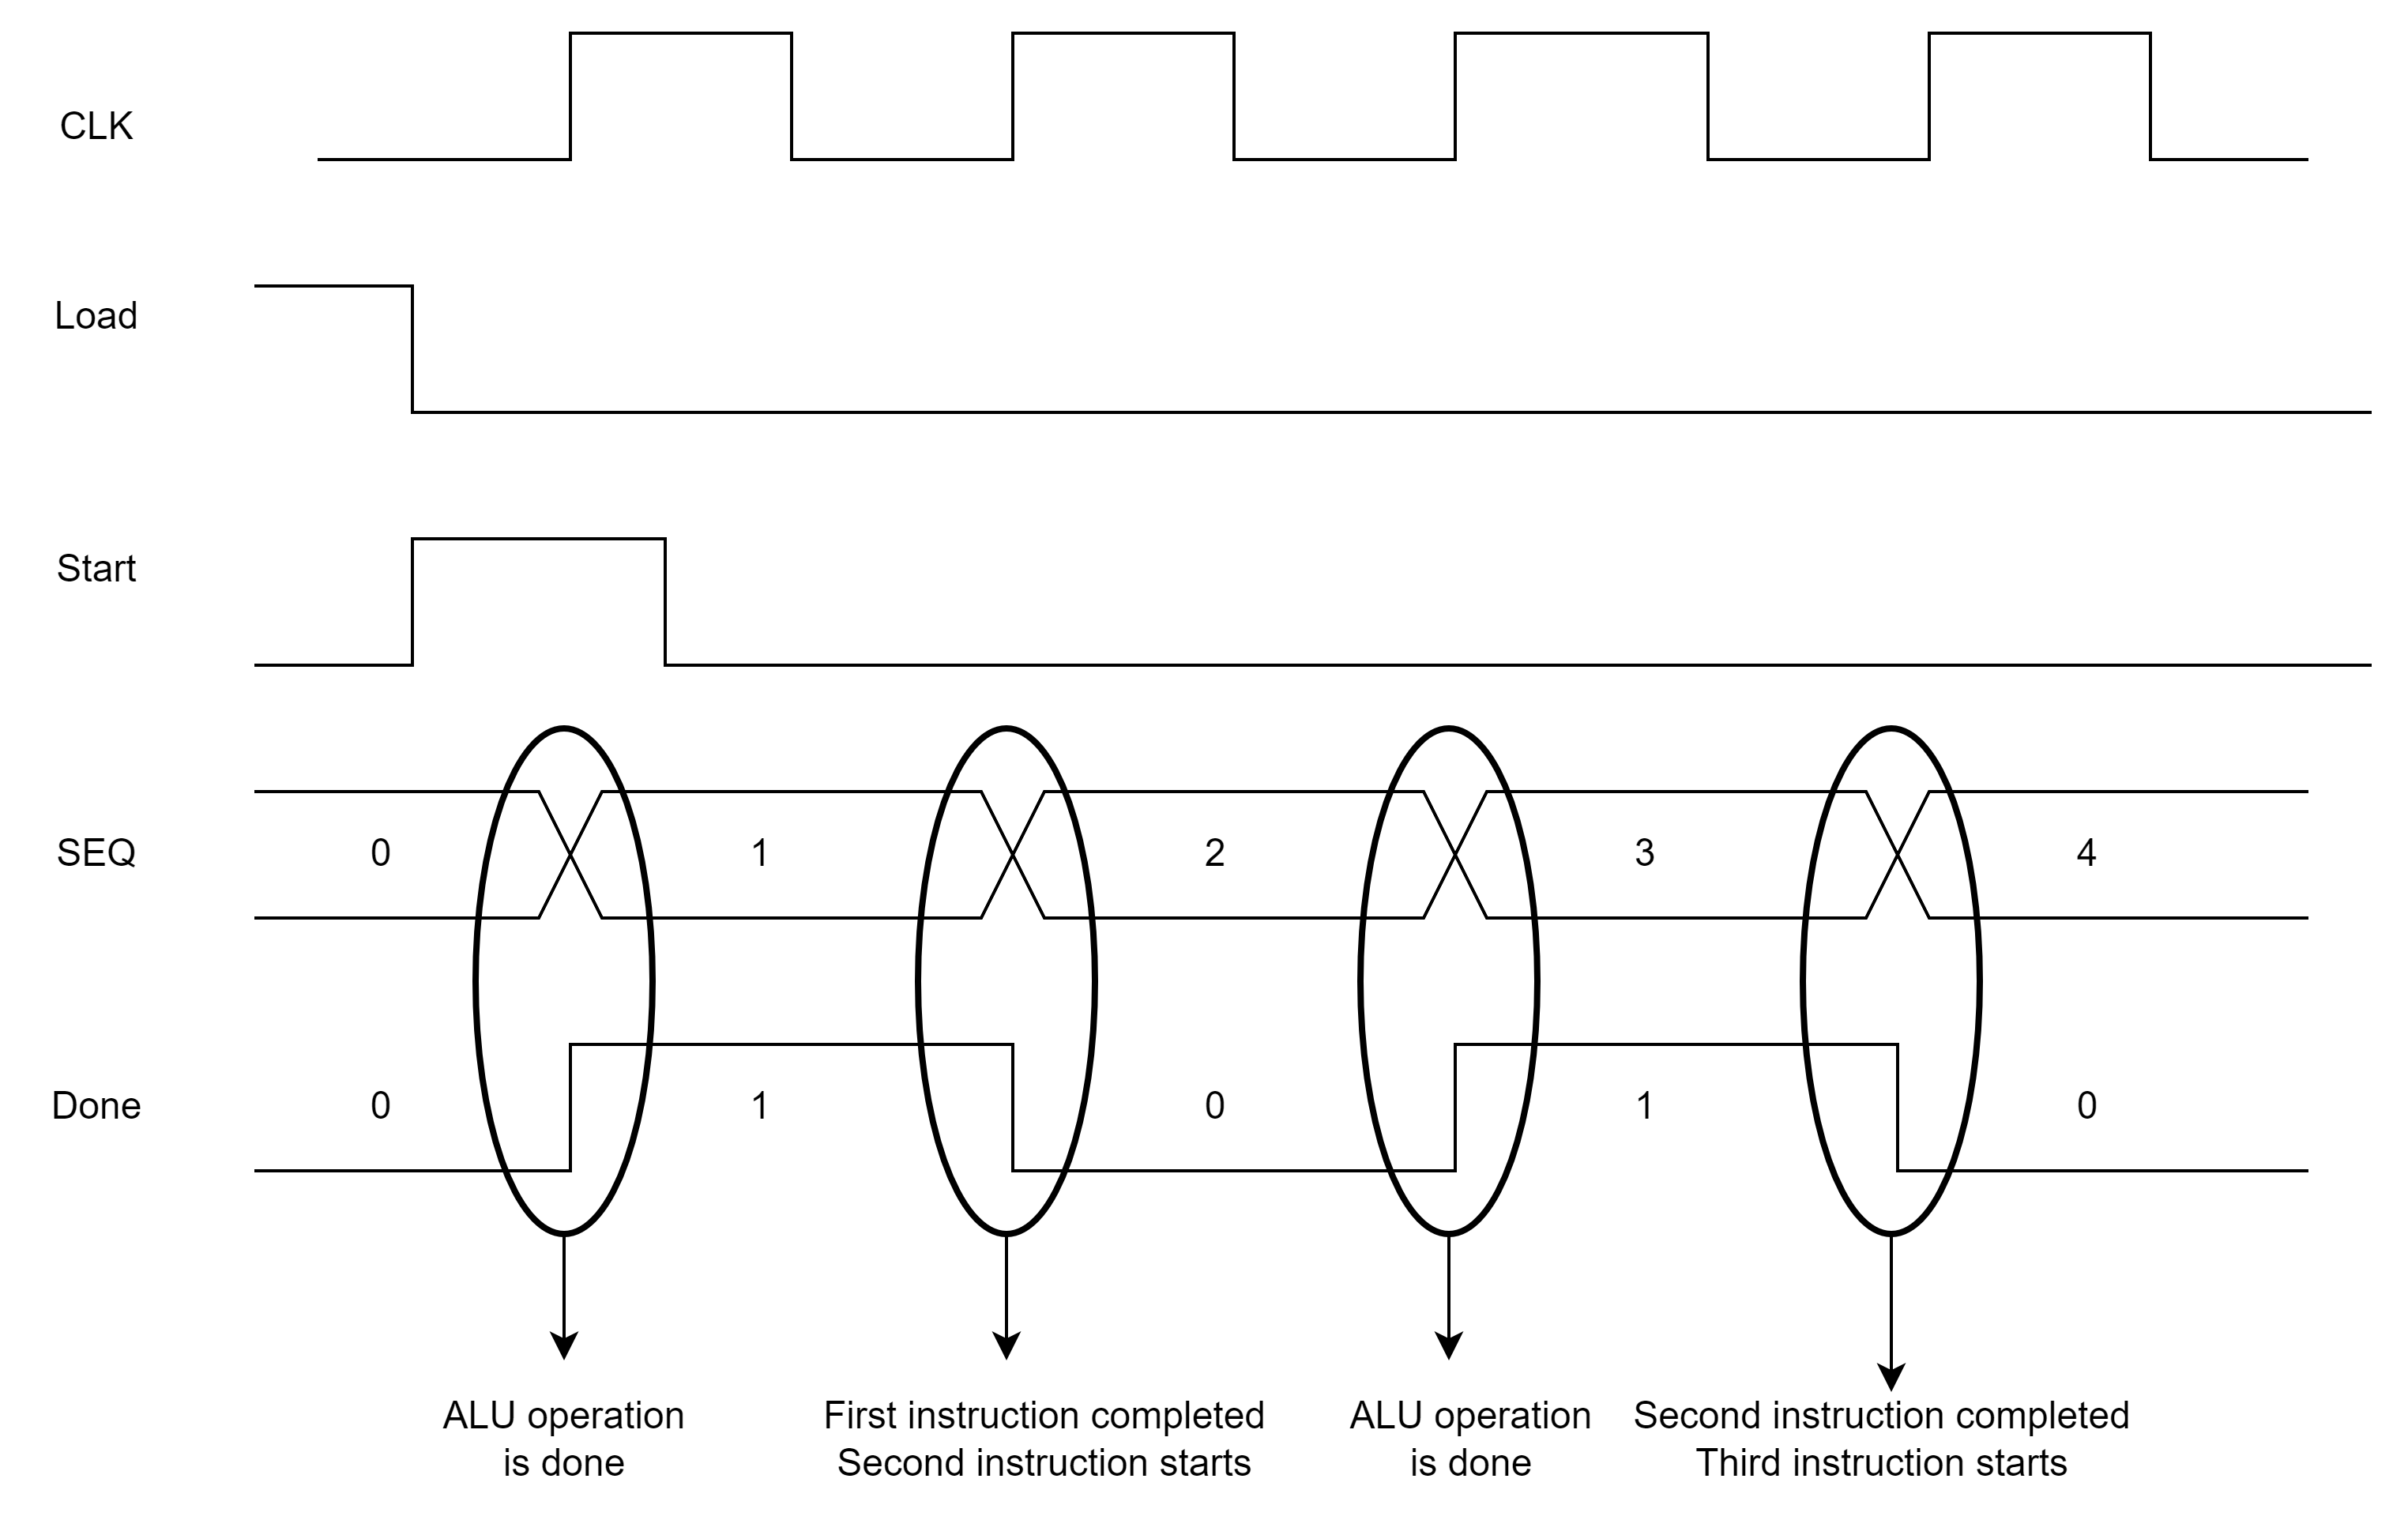
\includegraphics[scale=0.3]{timing.png}
\caption{Timing Design}
\label{timing}
\end{figure}
\end{landscape}


\newpage
\subsection*{Instruction Memory}
Instruction memory is the programmable part of the microcontroller. Instructions programmed to this memory is executed during the operation. The internal structure is straightforward and can be seen in Figure \ref{instr}. 

\begin{figure}[H]
\centering
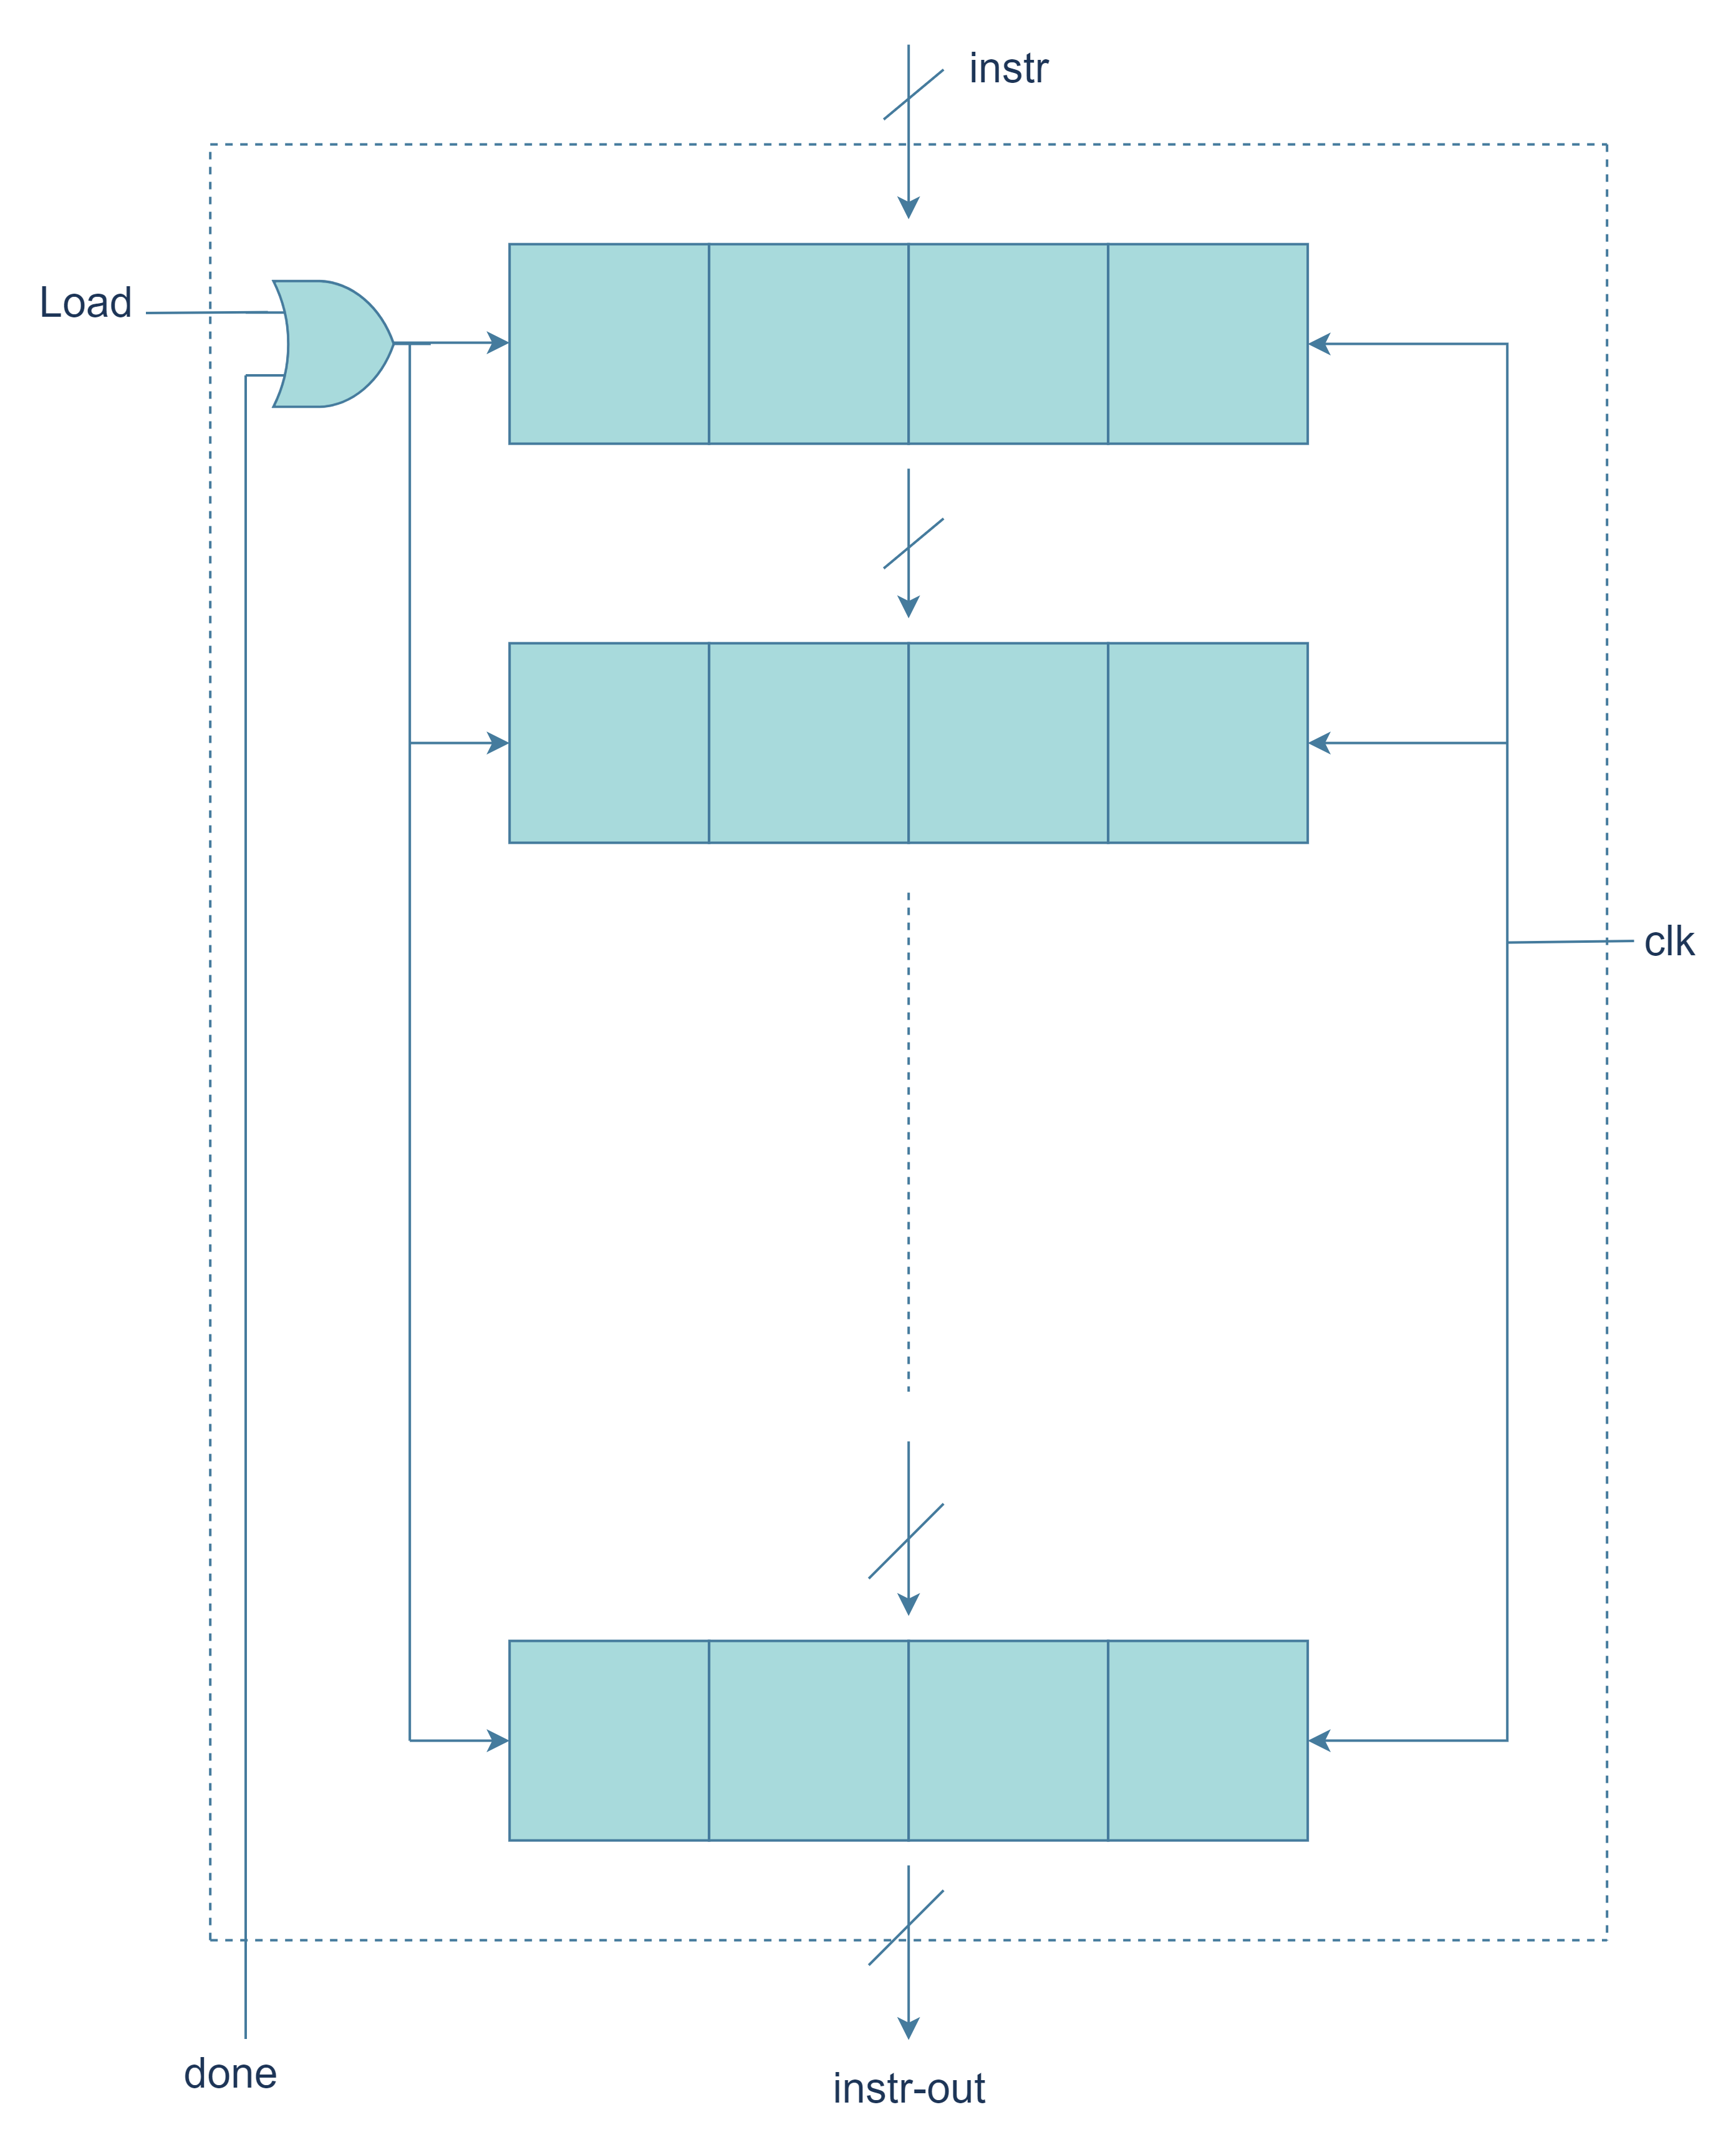
\includegraphics[scale=0.15]{instr.png}
\caption{Instruction Memory Architecture}
\label{instr}
\end{figure}


\begin{itemize}
\item There are eight 4-bit register which are connected in series. These eight registers should be loaded in 8 CLK cycles prior to the operation. External \textsl{Load} input should be ON during this interval. At each CLK cycle, registers change their contents and take the contents of the next register's contents.

\item Series shift of the instruction will be continued during the operation. When the \textsl{Done} signal is ON from the controller, load inputs of the register again activated and instructions slides down. Last register's content outputs to the controller.

\item \textbf{Alternative}: At the end of the operation, instruction memory is deleted totally. During the implementation, it is possible to add extra components to make a ring of registers to not lose the instructions during the operation.

\end{itemize}


\subsection*{Data Memory}

Data memory is a simple part. However, some important decisions are made and explained below. Diagram is shown in Figure \ref{data}.

\begin{figure}[H]
\centering
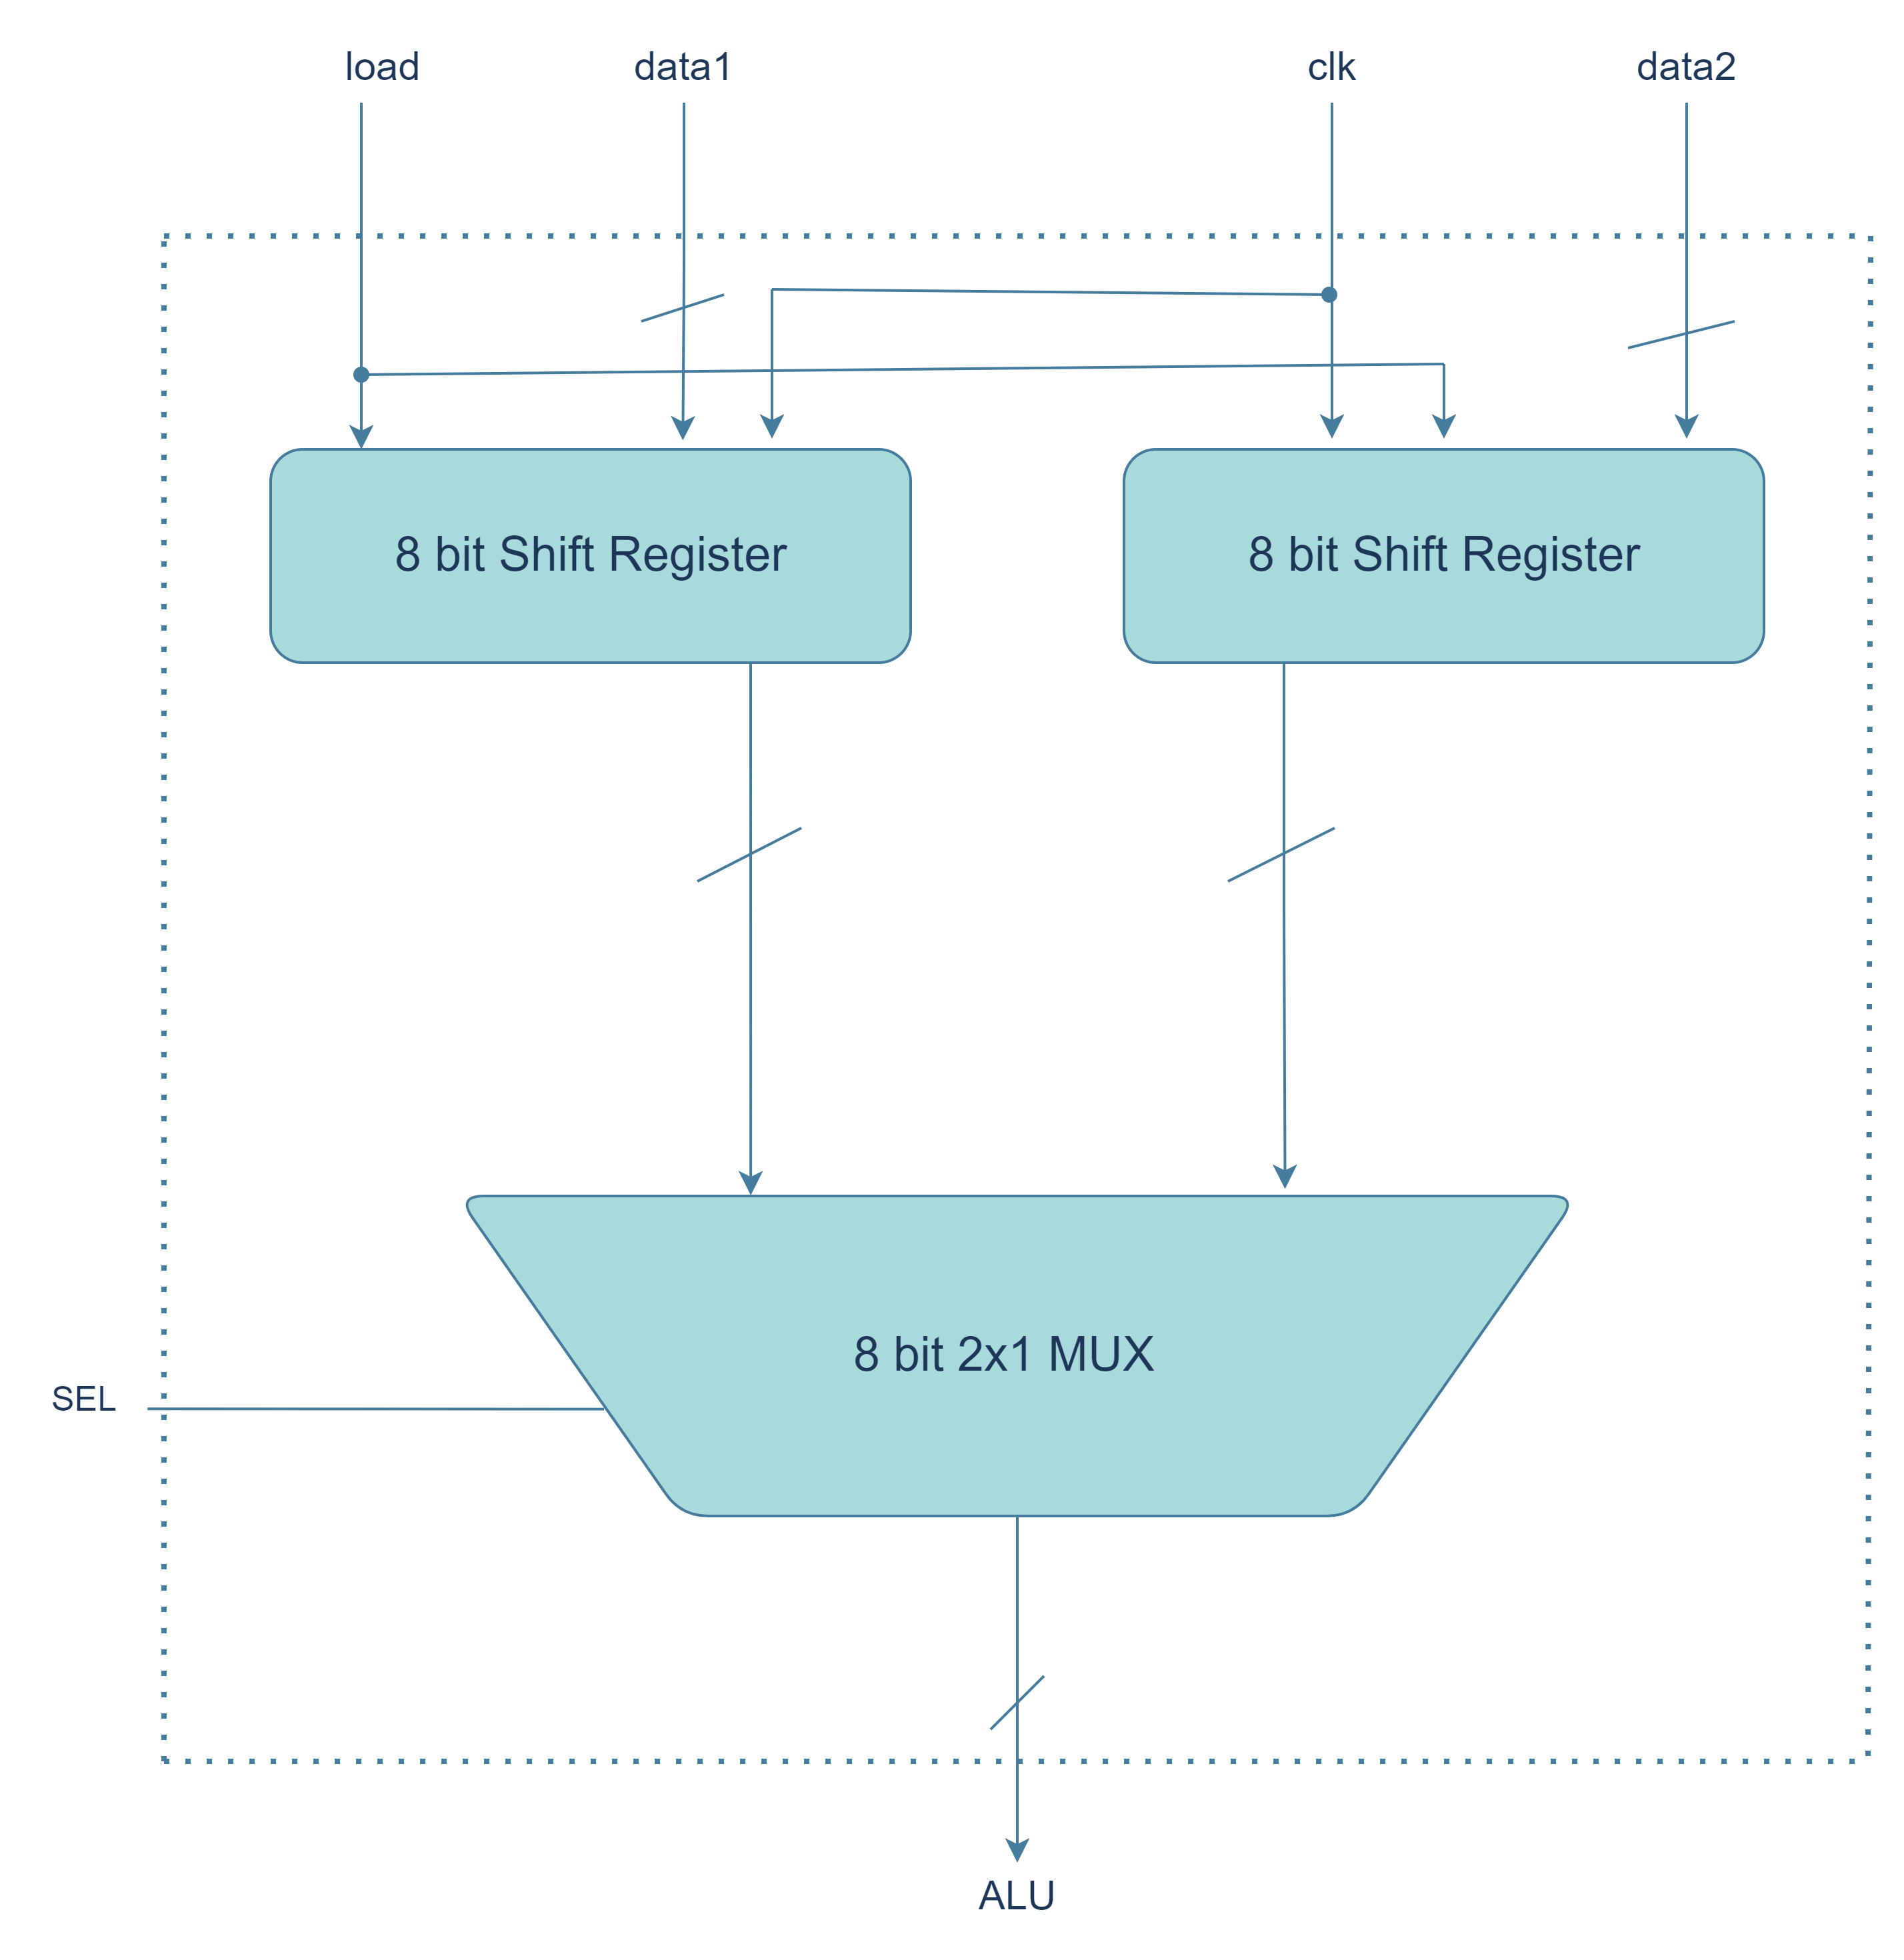
\includegraphics[scale=0.15]{data.png}
\caption{Data Memory Architecture}
\label{data}
\end{figure}


\begin{itemize}
\item Data memory takes two different 8-bit number and hold them until the end of operation. External \textsl{Load} signal is also responsible from the loading of the data memory.

\item A \textbf{very important design choice} is made during the  data memory design. That is, one 1-bit serial \textsl{data} input is replaced with two 1-bit serial input. These two serial input are to be routed to the \textsl{reg1} and \textsl{reg2}.\\
\underline{Reasoning:} Modern day computers is designed on uniformity and regularity motto \cite{b2}. Every instruction should be simple enough and take the same amount of time. Hence, all the operations follow the similar sequences and take similar time. In this view, I have decided to make the \textsl{data} input of this memory two serial input in order to:
\begin{itemize}
\item synchronize it with the instruction memory loading. We do not need to wait for another 8 CLK cycle for the data memory.
\item use the same \textsl{Load} signal from the external world. There is no need to have two different signal which is used for same purpose.
\end{itemize}


\item Output MUX select signal is controlled by the controller. According to the need of the current instruction, it chooses the \textsl{reg1} or \textsl{reg2}. This output directly goes to the ALU.
\end{itemize}


\subsection*{Controller}

Controller is the heart of the microcontroller. Other modules doesn't change much from a chip to chip. However, we should have a unique controller. Figure \ref{controller} shows the internal structure of the proposed controller.

\begin{figure}[H]
\centering
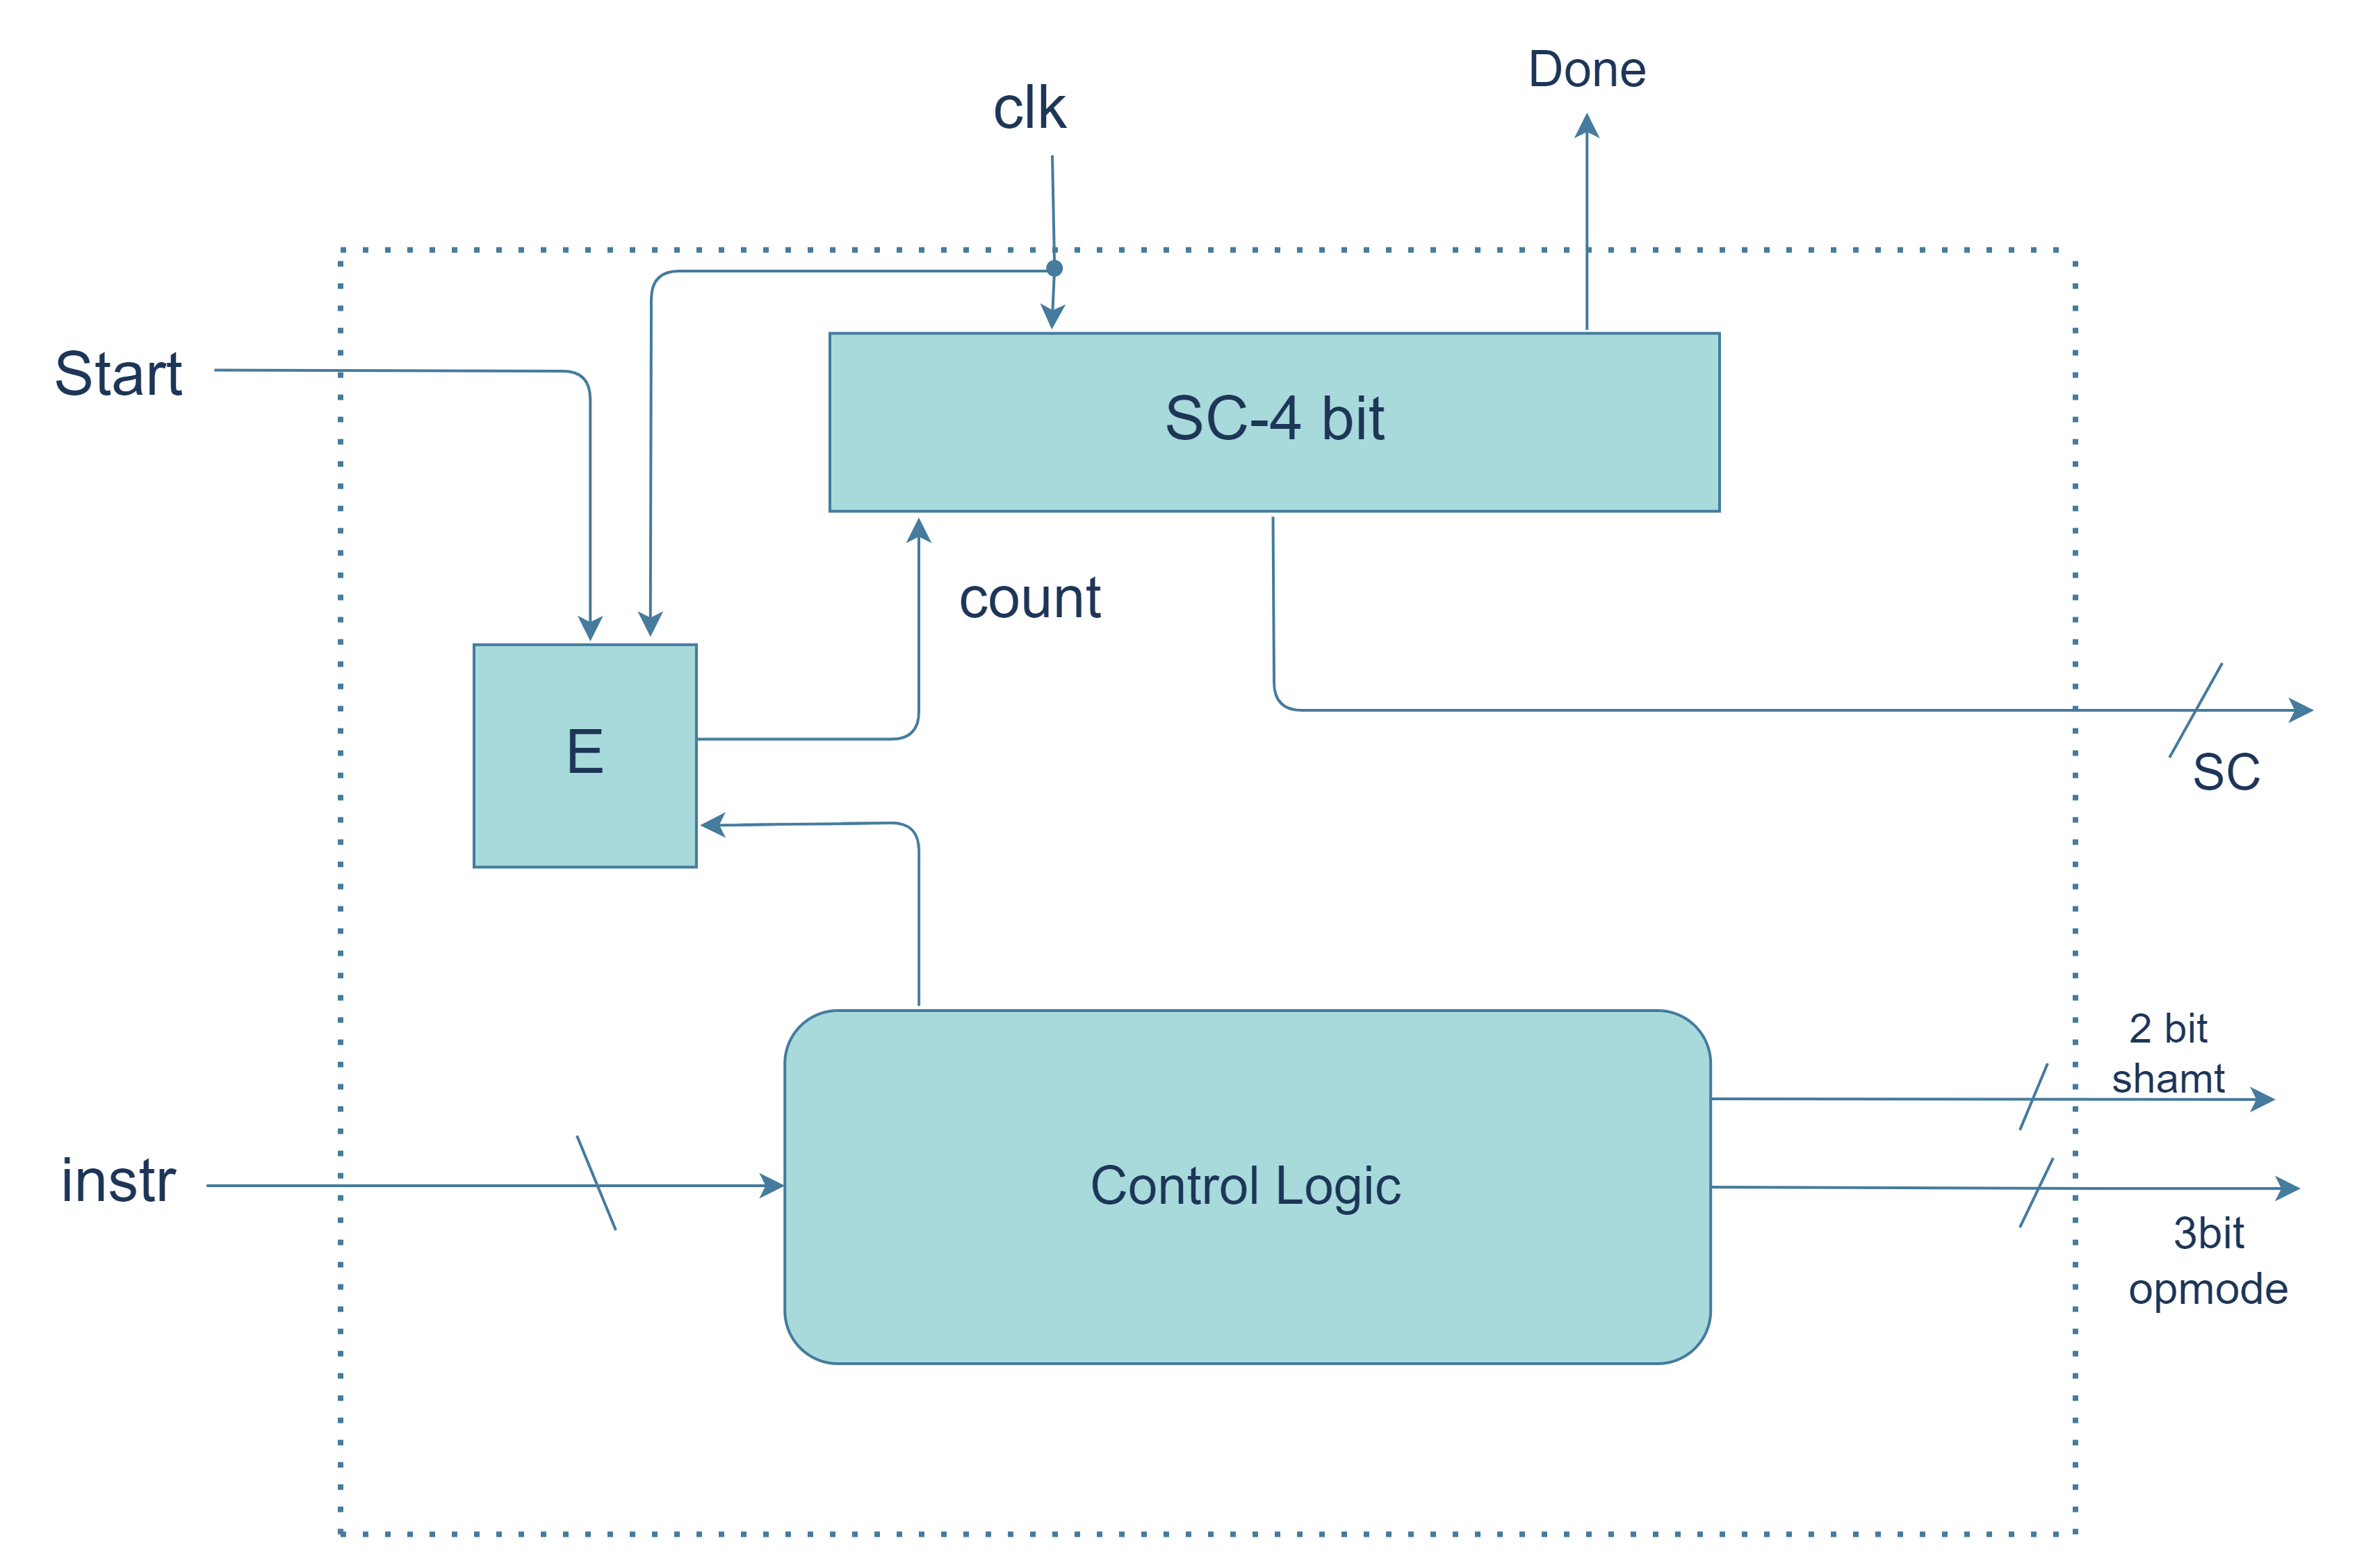
\includegraphics[scale=0.16]{controller.png}
\caption{Controller Architecture}
\label{controller}
\end{figure}

\begin{itemize}
\item Sequence counter is explained in detail in the timing section. Its count function is enabled by a single bit-register in the controller.

\item Single-bit register \textsl{E} stands for \textsl{Enable/End}. It looks for the \textsl{Start} signal and \textsl{End} instruction. When the operations starts it enables the sequence counter to count. End instruction ends this mode. Sequence counter is to be resetted.

\item Control logic takes the current instruction and produces the control signals for the data memory and ALU. 3 bit operation mode controls the operation of the ALU. After the careful considerations of the instructions, I could reduce the instruction set to the 8 simple operation. These can be summarized as follows:
\begin{enumerate}
\item Set
\item Reset 
\item Load \verb|ALU_in_1|
\item Load \verb|ALU_in_2|
\item Compared Load
\item Add \verb|ALU_in_1| + \verb|ALU_in_2|
\item Subtract \verb|ALU_in_1| - \verb|ALU_in_2|
\item Subtract \verb|ALU_in_2| - \verb|ALU_in_1|
\end{enumerate}
These eight different operation can be encoded in the 3-bit operation code (\textsl{opmode}).

\item Shift instructions is controlled independently by the 2-bit \textsl{shamt} control output from the controller. This signal is 2-bit because there are 3 different mode that should be captured:

\begin{enumerate}
\item No shift
\item Shift Right
\item Shift Left
\end{enumerate} 
\end{itemize}





\subsection*{Arithmetic Logic Unit}

Arithmetic Logic Unit provides the processing power of the microcontroller. Figure \ref{alu} shows the internal architecture of the arithmetic logic unit. There are 3 different submodules in this unit. 

\begin{figure}[H]
\centering
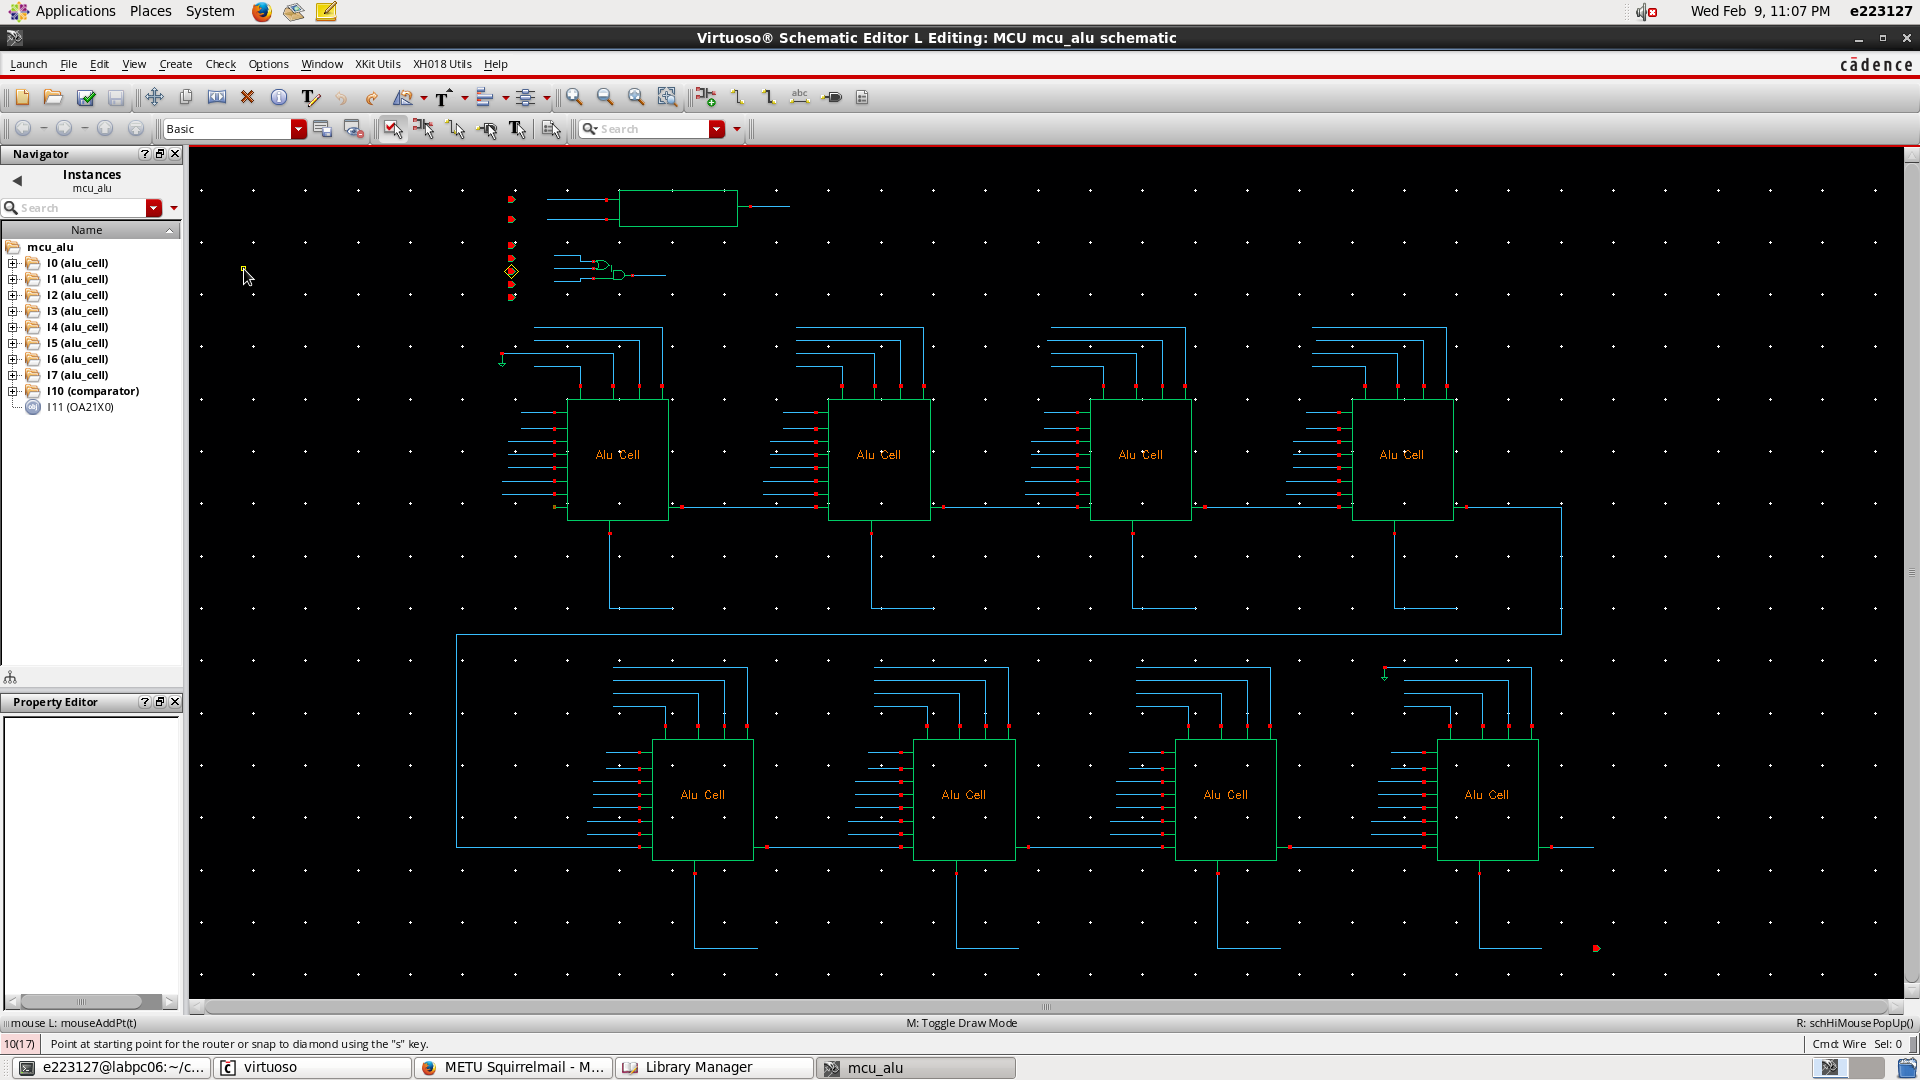
\includegraphics[scale=0.16]{alu.png}
\caption{Arithmetic Logic Unit Architecture}
\label{alu}
\end{figure}

\begin{itemize} 
\item \underline{\textsl{ALU subsystem}} is the core of the ALU unit. It performs most of the operation needed by the microcontroller. It can perform the following operations.
\begin{itemize}
\item Set
\item Reset 
\item Transfer
\item Add 
\item Subtract 
\end{itemize} 
ALU operation is controlled by 3-bit \textsl{opmode}. ALU operation is done with the help of 8-bit adder/subtractor and an output MUX to decide the operation. A possible adder/subtractor example is included in Figure \ref{adder} in the Appendix. Output is directly routed to the output RAM. It is written to the current address.

\item \underline{\textsl{Barrel Shifter}} is a combinational shifter circuit that can shift by any amount of bits in combinational domain. This is achieved using a brute force approach. All the possible connections are made to inputs of the MUXes. Necessary shift amount is dictated by the select inputs. It is rather easy to implement this structure in case of a 1-bit shift. Shift mode is controlled by the 2-bit \textsl{shamt} from the controller. One implementation example is in the Figure \ref{barrel} in Appendix which is taken from the Mano's book \cite{b1}. 

\item \underline{\textsl{8-bit Comparator}} compares the inputs and transfer this information to the ALU sub-unit. Comparison instructions use this information. Its output is 1 bit that shows the higher one of the inputs. There is no need of third case because in case of equality, choice is not critical. At this stage, there is no enable signal to the comparator. It works even if no comparison instructions are executed. In the implementation stage of the project, it is possible to add an enable signal to the comparator in order to increase the performance and reduce the extra capacitance delays. 

\item Data coming from the data memory is directly controlled inside the data memory as we have seen already. Therefore, there is no need to differentiate the \textsl{reg1} and \textsl{reg2} instructions in the ALU.
\end{itemize}




\subsection*{Output RAM}

The output unit of the microcontroller is the RAM. There are different approaches to RAM design. We all know the SRAM and DRAM approaches. These circuits are highly optimized for the best efficiency of the area. Therefore, their read/write operations are highly complicated. Due to the limited duration of project, it is hard to obtain a fully operational RAM structure. Precharge, sense circuitries and the cell design requires a long design and verification time. Therefore, I designed a new RAM unit. Figure \ref{ram} shows the internal structure of the RAM. Some explanations follows. 

\begin{itemize}
\item The proposed RAM structure is capable of doing everything standard RAMs do. It doesn't use the CLK input, so it's not a sequential circuit. We can reach each cell randomly whenever we want. Therefore, it is not a sequential memory.

\begin{figure}[H]
\centering
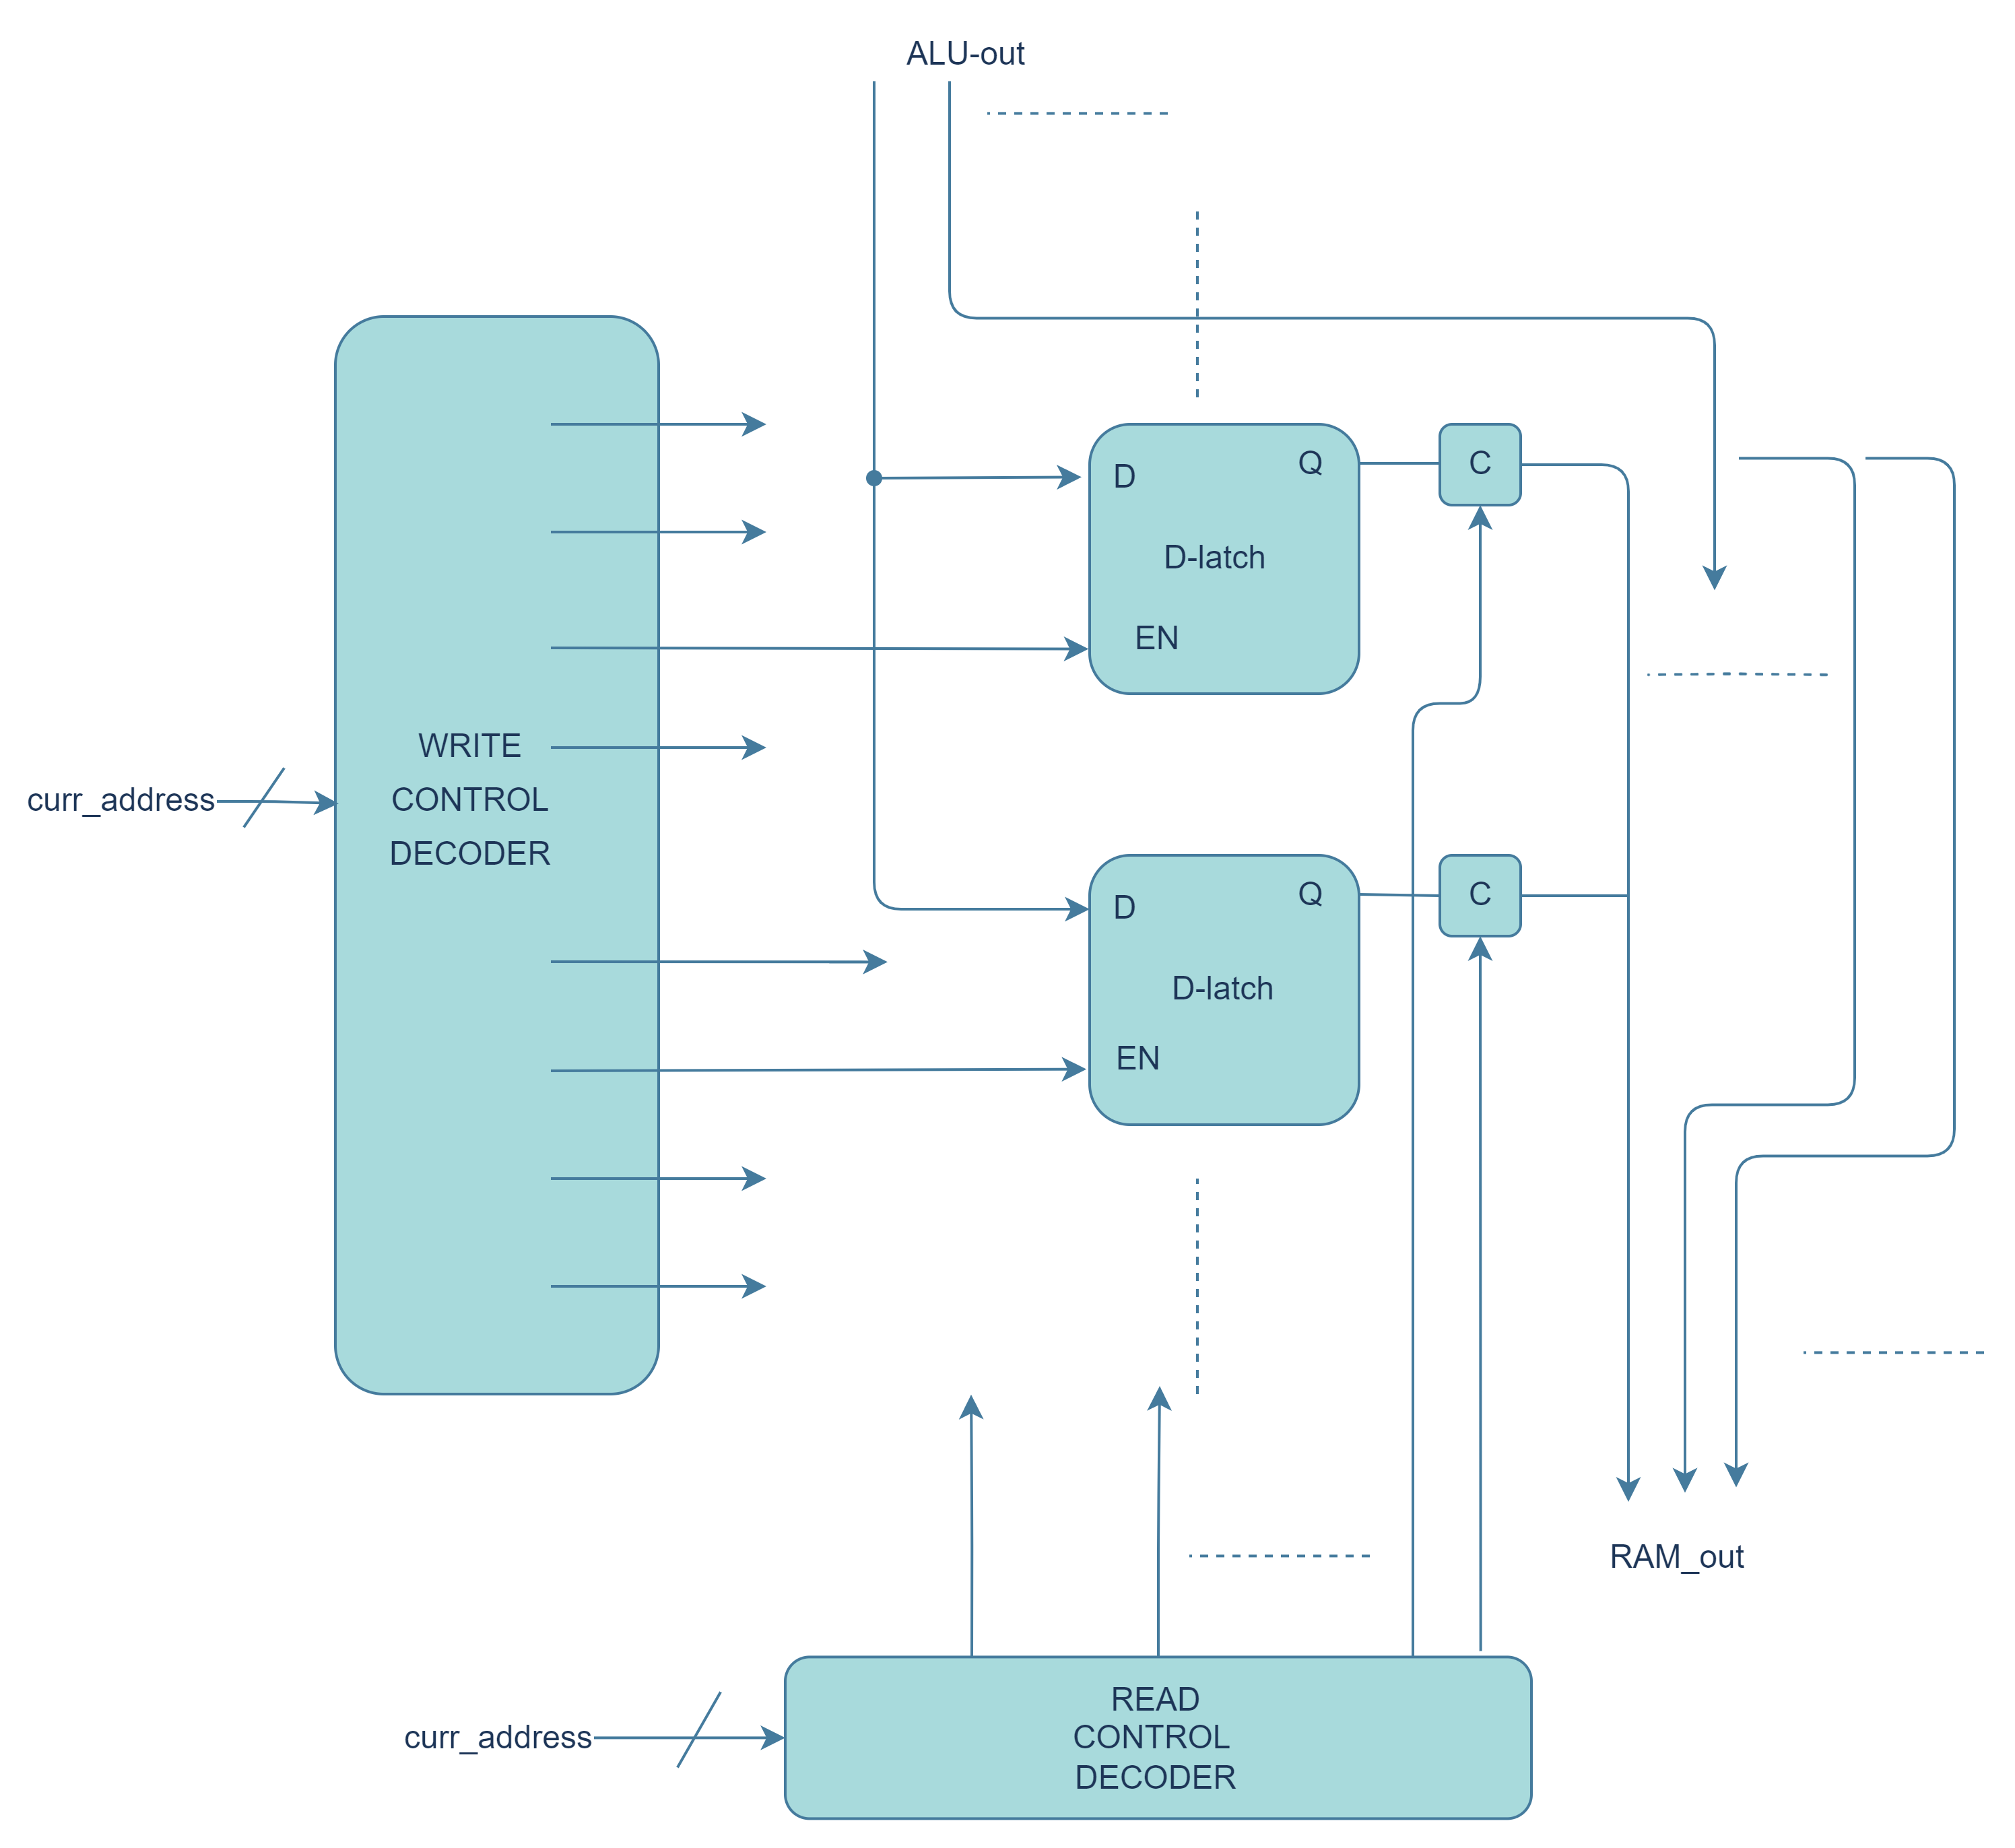
\includegraphics[scale=0.16]{ram.png}
\caption{Random Access Memory Architecture}
\label{ram}
\end{figure}



\item Read and Write signals and operations are separated from each other. Therefore, there is no bit-line shared between read and write. This gives us the ability to read and write at the same time. This feature allows 8-bit data from RAM to go to ALU without entering any register, and 8-bit input from ALU can be written directly to RAM.

\item Write signal is controlled with the \textsl{Write Control Decoder} which uses the current address register coming from the controller. Output of the decoder goes to the enable inputs of the desired word.

\item Standard 6T-SRAM structure -which is a latch of back to back inverters- is replaced with the D-latch due to the availability of the D-latch in the library. This increases the number of transistors.

\item \textsl{Read Control Decoder} also takes the current address input from controller. However, it is not a conventional decoder. It enables the previous address of the current address. This internal structure can be implemented easily using the standard decoder structure with additional gates. 

\item Output of the read decoder enables the transmission gates (complementary switch) at the output of D-latches shown with the C in the diagram. This structure is similar to the tri-state buffered bus structure. Only one bit can reach to the bit line.
\end{itemize}




\subsection*{Appendix}

\begin{figure}[H]
\centering
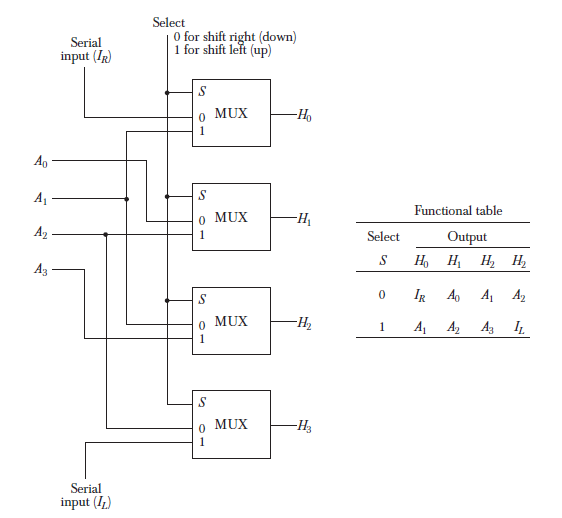
\includegraphics[scale=0.9]{barrel.png}
\caption{Combinational Barrel Shifter.         Source: \cite{b1}}
\label{barrel}
\end{figure}

\begin{figure}[H]
\centering
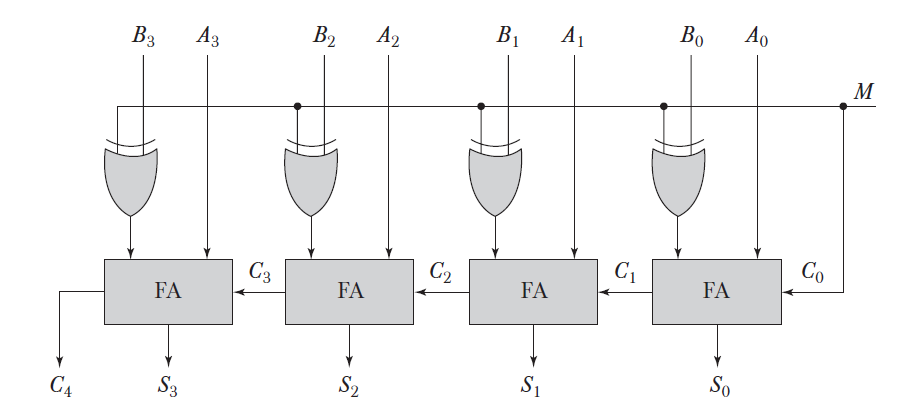
\includegraphics[scale=0.7]{adder.png}
\caption{A 4-bit Adder.     Source: \cite{b1}}
\label{adder}
\end{figure}




%%%%%%%% BIBLIOGRAPHY %%%%%%%%%%%%


\begin{thebibliography}{00}


\bibitem{b1} M. M. Mano, ``Register Transfer and Microoperations'' \emph{in Computer System Architecture}, New Delhi: Prentice-Hall of India, 2008, ch. 4, pp. 93-124.

\bibitem{b2} Sarah L. Harris and D. M. Harris, “Architecture,” in Digital Design and Computer Architecture, ARM ed., USA: Morgan Kaufmann, 2015, ch. 6, pp. 295–384. 

\end{thebibliography}



\end{document}
